%% Support sites:
%% http://www.michaelshell.org/tex/ieeetran/
%% http://www.ctan.org/tex-archive/macros/latex/contrib/IEEEtran/
%% and
%% http://www.ieee.org/

% Also note that the "draftcls" or "draftclsnofoot", not "draft", option
% should be used if it is desired that the figures are to be displayed in
% draft mode.
%
\documentclass[conference]{IEEEtran}
% Add the compsoc option for Computer Society conferences.

\usepackage{flushend}
%\usepackage{ifpdf}
\usepackage{cite}
\usepackage{pgfplots}
\usepackage{microtype}


%\usepackage{booktabs}

% *** GRAPHICS RELATED PACKAGES ***
%
\ifCLASSINFOpdf
  % \usepackage[pdftex]{graphicx}
  % declare the path(s) where your graphic files are
  % \graphicspath{{../pdf/}{../jpeg/}}
  % and their extensions so you won't have to specify these with
  % every instance of \includegraphics
  % \DeclareGraphicsExtensions{.pdf,.jpeg,.png}
\else
  % or other class option (dvipsone, dvipdf, if not using dvips). graphicx
  % will default to the driver specified in the system graphics.cfg if no
  % driver is specified.
  % \usepackage[dvips]{graphicx}
  % declare the path(s) where your graphic files are
  % \graphicspath{{../eps/}}
  % and their extensions so you won't have to specify these with
  % every instance of \includegraphics
  % \DeclareGraphicsExtensions{.eps}
\fi
% graphicx was written by David Carlisle and Sebastian Rahtz. It is
% required if you want graphics, photos, etc. graphicx.sty is already
% installed on most LaTeX systems. The latest version and documentation can
% be obtained at:
% http://www.ctan.org/tex-archive/macros/latex/required/graphics/
% Another good source of documentation is "Using Imported Graphics in
% LaTeX2e" by Keith Reckdahl which can be found as epslatex.ps or
% epslatex.pdf at: http://www.ctan.org/tex-archive/info/
%
% latex, and pdflatex in dvi mode, support graphics in encapsulated
% postscript (.eps) format. pdflatex in pdf mode supports graphics
% in .pdf, .jpeg, .png and .mps (metapost) formats. Users should ensure
% that all non-photo figures use a vector format (.eps, .pdf, .mps) and
% not a bitmapped formats (.jpeg, .png). IEEE frowns on bitmapped formats
% which can result in "jaggedy"/blurry rendering of lines and letters as
% well as large increases in file sizes.
%
% You can find documentation about the pdfTeX application at:
% http://www.tug.org/applications/pdftex

\usepackage[cmex10]{amsmath}
%\usepackage{amssymb}

% *** SPECIALIZED LIST PACKAGES ***
%
%\usepackage{algorithmic}
% algorithmic.sty was written by Peter Williams and Rogerio Brito.
% This package provides an algorithmic environment fo describing algorithms.
% You can use the algorithmic environment in-text or within a figure
% environment to provide for a floating algorithm. Do NOT use the algorithm
% floating environment provided by algorithm.sty (by the same authors) or
% algorithm2e.sty (by Christophe Fiorio) as IEEE does not use dedicated
% algorithm float types and packages that provide these will not provide
% correct IEEE style captions. The latest version and documentation of
% algorithmic.sty can be obtained at:
% http://www.ctan.org/tex-archive/macros/latex/contrib/algorithms/
% There is also a support site at:
% http://algorithms.berlios.de/index.html
% Also of interest may be the (relatively newer and more customizable)
% algorithmicx.sty package by Szasz Janos:
% http://www.ctan.org/tex-archive/macros/latex/contrib/algorithmicx/

\usepackage{listings}


\usepackage{array}
\usepackage{mdwmath}
\usepackage{mdwtab}

\usepackage{eqparbox}
%\usepackage[tight,footnotesize]{subfigure}
%\usepackage[caption=false]{caption}
\usepackage[caption=false, font=footnotesize]{subfig}
% subfig.sty, also written by Steven Douglas Cochran, is the modern
% replacement for subfigure.sty. However, subfig.sty requires and
% automatically loads Axel Sommerfeldt's caption.sty which will override
% IEEEtran.cls handling of captions and this will result in nonIEEE style
% figure/table captions. To prevent this problem, be sure and preload
% caption.sty with its "caption=false" package option. This is will preserve
% IEEEtran.cls handing of captions. Version 1.3 (2005/06/28) and later
% (recommended due to many improvements over 1.2) of subfig.sty supports
% the caption=false option directly:
%\usepackage[caption=false,font=footnotesize]{subfig}
%
% The latest version and documentation can be obtained at:
% http://www.ctan.org/tex-archive/macros/latex/contrib/subfig/
% The latest version and documentation of caption.sty can be obtained at:
% http://www.ctan.org/tex-archive/macros/latex/contrib/caption/




% *** FLOAT PACKAGES ***
%
%\usepackage{fixltx2e}
% fixltx2e, the successor to the earlier fix2col.sty, was written by
% Frank Mittelbach and David Carlisle. This package corrects a few problems
% in the LaTeX2e kernel, the most notable of which is that in current
% LaTeX2e releases, the ordering of single and double column floats is not
% guaranteed to be preserved. Thus, an unpatched LaTeX2e can allow a
% single column figure to be placed prior to an earlier double column
% figure. The latest version and documentation can be found at:
% http://www.ctan.org/tex-archive/macros/latex/base/



%\usepackage{stfloats}
% stfloats.sty was written by Sigitas Tolusis. This package gives LaTeX2e
% the ability to do double column floats at the bottom of the page as well
% as the top. (e.g., "\begin{figure*}[!b]" is not normally possible in
% LaTeX2e). It also provides a command:
%\fnbelowfloat
% to enable the placement of footnotes below bottom floats (the standard
% LaTeX2e kernel puts them above bottom floats). This is an invasive package
% which rewrites many portions of the LaTeX2e float routines. It may not work
% with other packages that modify the LaTeX2e float routines. The latest
% version and documentation can be obtained at:
% http://www.ctan.org/tex-archive/macros/latex/contrib/sttools/
% Documentation is contained in the stfloats.sty comments as well as in the
% presfull.pdf file. Do not use the stfloats baselinefloat ability as IEEE
% does not allow \baselineskip to stretch. Authors submitting work to the
% IEEE should note that IEEE rarely uses double column equations and
% that authors should try to avoid such use. Do not be tempted to use the
% cuted.sty or midfloat.sty packages (also by Sigitas Tolusis) as IEEE does
% not format its papers in such ways.


\usepackage{url}
\usepackage{epstopdf}



% *** Do not adjust lengths that control margins, column widths, etc. ***
% *** Do not use packages that alter fonts (such as pslatex).         ***
% There should be no need to do such things with IEEEtran.cls V1.6 and later.
% (Unless specifically asked to do so by the journal or conference you plan
% to submit to, of course. )


% correct bad hyphenation here
\hyphenation{op-tical net-works semi-conduc-tor}

\usepackage[normalem]{ulem}
\usepackage{tikz}
\usepackage{xcolor}
\usepackage{lipsum}
\usepackage{verbatim}
\usepackage{multirow}
\usepackage{multicol}
\usetikzlibrary{shapes,arrows,fit}

\tikzstyle{decision} = [diamond, draw, fill=blue!20, text width=4.5em,
text badly centered, node distance=3cm, inner sep=0pt]

\tikzstyle{block} = [rectangle, draw, fill=blue!20, text width=5em,
text centered, rounded corners, minimum height=4em]

\tikzstyle{line} = [draw, -latex'] \tikzstyle{cloud} = [draw,
ellipse,fill=red!20, node distance=3cm, minimum height=2em]

\newcommand{\XXX}[1]{{\bf \color{red} XXX: #1}}
\newcommand{\TODO}[0]{{\bf \color{red} TODO\ }}
\newcommand{\MAXC}[0]{FAST}
\newcommand\reduline{\bgroup\markoverwith
  {\textcolor{red}{\rule[-0.5ex]{2pt}{0.4pt}}}\ULon}
\newcommand{\FIC}[1]{\reduline{#1}}
\newcommand{\blt}{\raise .2ex\hbox{\tiny$\bullet$ }}

%\usepackage[margin=1cm]{caption}

\newcounter{nodemarkers}
\newcommand\marktext[1]{%
    \tikz[overlay,remember picture]
        \node (marker-\arabic{nodemarkers}-a) at (0,1.5ex) {};%
    #1%
    \tikz[overlay,remember picture]
        \node (marker-\arabic{nodemarkers}-b) at (0,0){};%
    \tikz[overlay,remember picture,inner sep=2pt]
        \node[draw,dotted,rectangle,fit=(marker-\arabic{nodemarkers}-a.center) (marker-\arabic{nodemarkers}-b.center)] {};%
    \stepcounter{nodemarkers}%
}

\begin{document}

\captionsetup{width=2cm}

\lstdefinestyle{lara}{ language=C++, breaklines=true, % frame=tb,
  xleftmargin=2em, numbers=left, captionpos=b,
  morekeywords={aspectdef, var, apply, select, condition, begin, end, input} }

\lstdefinestyle{MaxC}{language=C++, breaklines=true, %frame=tb,
  xleftmargin=2em, numbers=left,
  captionpos=b,basicstyle=\ttfamily\footnotesize,
  morekeywords={s_int32, int32, float8_24, sin_float8_24,
    sout_float8_24, float8_24, s_int, s_float8_24, s_bool},
    deletekeywords={static}}

\title{Aspect Driven Compilation for \\ Dataflow Designs}

\author{
  \IEEEauthorblockN{
    \emph{Paul Grigora\c{s}}\IEEEauthorrefmark{1},
    \emph{Xinyu Niu}\IEEEauthorrefmark{1},
    \emph{Jose G. F. Coutinho}\IEEEauthorrefmark{1},
    \emph{Wayne Luk}\IEEEauthorrefmark{1},
    \emph{Jacob Bower}\IEEEauthorrefmark{2} and
    \emph{Oliver Pell}\IEEEauthorrefmark{2} \vspace{0.1cm}
  }
  \IEEEauthorblockA{
    \IEEEauthorrefmark{1}
    Department of Computing, Imperial College London, 180 Queen's Gate, London SW7 2AZ, UK
  }
  \IEEEauthorblockA{
    \IEEEauthorrefmark{2}Maxeler Technologies Ltd, 1 Down Place, London W6 9JH, UK
   }
  \IEEEauthorblockA{
   Email: \{paul.grigoras09, niu.xinyu10, gabriel.figueiredo, w.luk\}@imperial.ac.uk, \{jacob, oliver\}@maxeler.com
  }
}

\maketitle

\begin{abstract}
This paper describes a novel approach for implementing designs with
run-time reconfiguration on FPGAs using a dataflow approach to
increase performance. We introduce features of the FAST language that
support static reconfiguration in which the partitions are determined
at compilation time. Aspect-driven synthesis is used to generate more
advanced designs that are self-adaptive, being able to choose between
multiple existing configurations to improve performance. We evaluate
our approach by implementing two high-performance designs for Reverse
Time-Migration and Barrier Option pricing.
\end{abstract}


\IEEEpeerreviewmaketitle

\section{Introduction}
We identify the following challenges:
\begin{itemize}
\item supporting run-time reconfiguration in an intutitive and simple
  fashion; current tools require explicit, complicate API calls to achieve
\item supporting self-adaptability in run-time reconfigurable designs;
\end{itemize}

Our contributions include:
\begin{itemize}
\item we introduce and implement extensions/features of the FAST
  language that support static run-time reconfiguration
\item we introduce aspects in LARA that can be used to generate
\end{itemize}

\section{Design Flow}
\label{sec:design-flow}

To improve both efficiency and productivity, our design flow focuses
on maintaining or improving the \emph{performance} and \emph{energy
  efficiency} of existing applications while using a more systematic
approach for design optimisation that results in more \emph{portable}
application code, improves \emph{integration} with existing
applications and \emph{automates} manual, time consuming and
error-prone tasks.

\begin{comment}
Our design flow aims to improve both \emph{efficiency} (in terms of
performance and energy consumption) and \emph{productivity}. The
former is crucial to High Performance Computing, the latter helps
reduce development cost and time and is a well-known issue with
existing FPGA based acceleration solutions \cite{jones2010gpu}. To
achieve this we focus on maintaining or improving the
\emph{performance} and \emph{energy efficiency} of existing
applications while using a more systematic approach for design
optimisation that results in more \emph{portable} application code,
improves \emph{integration} with existing applications and
\emph{automates} manual, time consuming and error-prone tasks.
\end{comment}

The key components of the design flow are:
\begin{itemize}
\item \emph{\FAST{}}, a novel language for specifying dataflow designs
  which is compatible with C syntax, improving developer productivity
  and supporting combined hardware and software specifications;

\item \emph{aspect driven compilation flow}, used to decouple
  optimisation from design development, improving design portability,
  and automating the generation of code and design space
  exploration~\footnote{the process of exploring multiple
    configurations to identify optimal implementations} which improves
  productivity;

\item \emph{systematic design space exploration}, to identify maximum
  performance configurations by using \emph{aspect descriptions} to
  conveniently control and guide the exploration process based on
  user-specified constraints;
\end{itemize}

\Cref{fig:design-flow} illustrates the design flow:
\begin{enumerate}
\item a C application containing an embedded high-level dataflow
  design specified in \FAST{} is developed from the original source
  application;
\item the dataflow design is transformed by the aspects in the
  repository to generate new configurations (e.g. with multiple
  word-length configurations);
\item the generated configurations are compiled using a backend
  compilation toolchain (MaxCompiler) to dataflow designs
  implemented on FPGAs;
\item the feedback from the compilation process is used to drive
  design space exploration, repeating the weaving and compilation
  process until user-specified constraints are satisfied.
\end{enumerate}

\begin{figure}[!ht]
  \centering
  \def\svgwidth{0.8\linewidth}
  \input{figs/asap13-design-flow.pdf_tex}
  \caption{Proposed approach for aspect-driven compilation of dataflow
   designs.}
  \label{fig:design-flow}
\end{figure}
\section{The \MAXC{} Language}
\label{sec:maxc}

\MAXC{} (Facile Aspect-driven Source Transformation) is a novel
language for specifying dataflow designs that are used as a starting
point for the design flow proposed in Section
\ref{sec:design-flow}. In particular, we use C syntax to capture
dataflow computations, and, instead of heavily relying on API libraries
to specify the design (as in MaxCompiler \cite{5719584} or Streams-C
\cite{Gokhale:Stone:Arnold:Kalinowski:2000}), we use aspects to
implement the transformations required for the actual implementation.

\MAXC{} provides the following features that are
required by the proposed flow:

\begin{itemize}
\item \emph{Imperative specification of dataflow designs}. C99 syntax is
  enforced by the \MAXC{} compiler which is based on the ROSE
  Framework (with EDG as a front-end) and makes the language familiar
  and easy to adopt for developers, facilitating translation of
  existing application code to dataflow designs.
\item \emph{Good integration with existing source level translation and
  weaving tools}. Simple syntax allows the language to interact well
  with existing compilers or source to source translation frameworks,
  allowing source level optimisations to be applied through different
  tools.
\item \emph{Combined hardware/software design}. Specifications of dataflow
  kernels and CPU run-time software can be mixed. The example shown in
  Fig.~\ref{fig:maxc-1dconv} can be compiled with the GCC toolchain,
  but when using the \MAXC{} compiler, the pragma indicates the link
  between the software and hardware, which results in an accelerated
  hardware software/solution.
\item \emph{Support for data path and control path generation}. \MAXC{}
  allows specifying both data and control operations that are
  automatically mapped to stream multiplexers.
\end{itemize}

\MAXC{} is used to express the simplest form of a dataflow design
while optimisations and other transformations are encapsulated in
aspects which are developed separately and applied through aspect
weaving. This results in a flexible approach for generating and
exploring the space of efficient dataflow designs.

Designs in \MAXC{} are compiled to MaxCompiler designs composed of
inter-connected functional kernels. Communication between kernels is
asynchronous, so they can operate independently, and compute only when
all active inputs have available data.

Table~\ref{table:maxc-features} summarises the features of \MAXC{} and
Fig.~\ref{fig:maxc-1dconv} shows an example dataflow kernel used to
value European options. Kernels are defined as regular C functions
with inputs clearly defined as arguments in the function
signature. Streams are represented as regular C99-style pointers.
Normal array notation can be used to generate either previous or
future values or dereference the stream to obtain the current stream
value. Negative indices are allowed for accessing previous stream
values and supported offset expressions are linear expressions
comprised of constants or variables (either loop induction variables,
or normal variables but for which a compile time range of values is
specified -- this is required to generate efficient
hardware). Constructs such as loops are supported as long as their
bounds are known at compile time and are used to parametrize dataflow
designs with values known at compilation time.

\begin{table}[!h]
  \centering
\renewcommand{\arraystretch}{1.6}
\caption{Summary of the main features of the \MAXC{} language.}
\label{table:maxc-features}
\begin{tabular}{p{1.7cm}|l|l}
\hline
\bf{Feature}                   & \bf{Description}                   & \bf{Method (see Fig.~\ref{fig:maxc-1dconv})} \\
\hline\hline
  \multirow{2}{*}{Input/Output}         & Declared in function header          & C99 (line 1)                                 \\\cline{2-3}       & \texttt{in()},\texttt{out()}  & \MAXC{} API (lines 2,11) \\
\hline
  \multirow{2}{*}{Control}     & Ternary op., \texttt{if} statement & C99 (line 11)                                \\\cline{2-3}      & Stream mux (\texttt{mux()})       & \MAXC{} API  \\
\hline
\multirow{2}{*}{Computation} & +, *, /, -                         & C99 (line 8)                           \\\cline{2-3} & log, exp, sqrt, sin etc.  & \#include $<$math.h$>$  \\
\hline
  \multirow{2}{*}{Streams}     & Declared as pointers               & C99 (line 1)                                 \\\cline{2-3}       & Accessed with array index & C99 (line 8) \\
\hline
  Optimisation                 & C pragmas                   & C99 (line 7)                                 \\
\hline
  Parameterization             & Constants, variables                   & C99                                          \\
\hline
Hardware \  Mapping                  & C pragmas                   & C99 (line 17)                                \\
\end{tabular}
\end{table}



\lstset{style=MaxC}

\begin{figure}[!h]
  \begin{lstlisting}
    void Price_FPGA(float* p, float c_0_0_0, float c_p_0_0, float c_n_0_0, int n1, int ORDER) {
      in(p);

      float* i4 = count(1000, 1);
      float* i1 = countChain(n1, 1, i4);

      #pragma FAST DSPBalance:full
      int result = p[0]  * c_0_0_0 + p[1]  * c_p_0_0 + p[-1] * c_n_0_0;

      int up =(i1 >= ORDER) && (i1 < n1 - ORDER);
      out(up ? result : p);
    }

    void Price_CPU(...) {...}

    int main() {
      #pragma FAST hw:Price_FPGA
      Price_CPU(...);
    }
  \end{lstlisting}
  \caption{\MAXC{} dataflow kernel for European Options
    pricing.}
  \label{fig:maxc-1dconv}
\end{figure}


The \MAXC{} API provides higher-level constructs such as I/O functions
(\texttt{in()}, \texttt{out()}), counters (Fig.~\ref{fig:maxc-1dconv},
Lines 4--5) and functions to multiplex streams (\texttt{mux()}). C
function calls are mapped to dataflow kernels via pragmas (Line 17)
which provides the flexibility of selecting a particular dataflow
configuration based on run-time conditions. Support for run-time
reconfiguration is included but will be described in a future
publication due to lack of space.

\section{Aspect Descriptions}
\begin{frame}
  \frametitle{Aspect Descriptions}
\begin{enumerate}
  \item  system aspect descriptions (e.g. monitor performance)
  \item implementation aspect descriptions (e.g. optimise word-length for operators)
  \item exploration aspect descriptions (e.g. control automation of design space exploration)
  \item development aspect descriptions (e.g. assist debugging)
\end{enumerate}

\end{frame}


\begin{frame}
  \frametitle{System Aspects}
Hardware/Software Partitioning:
\begin{enumerate}
  \item detect hotspots
  \item detect code patterns suitable for acceleration
  \item perform outlining transformation
  \item derive dataflow \texttt{fast\_f()} from \texttt{f()}
  \item place FAST pragma to link \texttt{fast\_f()} with \texttt{f()}
\end{enumerate}
\end{frame}


\begin{frame}[fragile]
  \frametitle{System Aspects: Monitoring}
  For all innermost loops:
\begin{itemize}
  \item Monitor every loop iteration
  \item Monitor every loop entry and exit
\end{itemize}
\begin{lstlisting}[label=lst:label, style=lara]
aspectdef LoopMonitor
  function.loop{is_innermost}:
    entry:   prepend(mon_iterationIn());
    exit :   append (mon_iterationOut());
    default: prepend(mon_instanceIn());
             append(mon_instanceOut());
end
\end{lstlisting}
\end{frame}

\begin{frame}
  \frametitle{Monitorisation: Aspect Weaving}
\begin{center}
\renewcommand{\arraystretch}{1.2}
\begin{tabular}{p{5cm}|p{5cm}}
\hline
\bf{Original Code}           & \bf{Woven Code}                                   \\
\hline
void f() \{                  & void f() \{                                       \\
                             & \hspace{3ex}\emph{monitor\_instanceI("f:1");} \\
\hspace{3ex}while (i $ < $ N) \{ & \hspace{3ex}while (i$ < $N) \{                      \\
                             & \hspace{6ex}\emph{monitor\_iterI("f:1");}     \\
\hspace{6ex}i++;             & \hspace{6ex}i++;                                  \\
                             & \hspace{6ex}\emph{monitor\_iterE("f:1");}     \\
\hspace{3ex}\}               & \hspace{3ex}\}                                    \\
                             & \hspace{3ex}\emph{monitor\_instanceE("f:1");} \\
\}                           & \}                                                \\
\end{tabular}
\end{center}
\end{frame}

\begin{frame}{System Aspects: Run-time Reconfiguration}
Explain why run-time reconfiguration is useful
\end{frame}

\begin{frame}{System Aspects: Run-time Reconfiguration}
Show aspects for run-time reconfiguration and general strategy
\end{frame}

\begin{frame}[fragile]{Implementation Aspects: Operator Optimisation}
\begin{lstlisting}[label=lst:label, style=lara]
aspectdef DspBalancing
var op_granularity =
 [{DspBalance:’full’,MultiplyOp: 5,AddOp: 5 },
  {DspBalance:’balanced’,MultiplyOp:3}];

select function.statement end
apply
 for (var i in op_granularity) {
   var gprofile = op_granularity[i];
   var match = true;
   for (var k in gprofile) {
     if (k != ’DspBalance’) {
       match &= ($statement.num_construct(k)
                 >= gprofile[k]);}}
   if (match) {
     var pragma = ’#pragma FAST balanceDSP:’
                   + gprofile.DspFactor;
     $statement.insert before "[[pragma]]";
     break;}}
   end
end
\end{lstlisting}
\end{frame}

\begin{frame}[fragile]{Exploration Aspects: Control DSE}
\begin{lstlisting}[label=lst:label, style=lara]
aspectdef DesignExploration
  input
   attribute,
   start, step,
   resource, resource_threshold,
   config
end
config[attribute] = start;
var i = 0;
do {
  var designName = genName(config);
  call genFAST(designName, config);
  buildFAST(designName);
  config[attribute] += step; i++;
} while (@hw[designName]. resource < resource_threshold && i < LIMIT);
end
\end{lstlisting}
\end{frame}

\begin{frame}[fragile]{Development Aspects: Debugging}
\begin{lstlisting}[label=lst:label, style=lara]
aspectdef WatchVar
select function.vref end
apply
  $vref.parent_stmt.insert before
  %{ log("[[$vref.name]]", [[$vref.name]]); }%
  $vref.parent_stmt.insert after
  %{ log("[[$vref.name]]", [[$vref.name]]); }%
end
condition $vref.is_out end
end
\end{lstlisting}

\begin{itemize}
\item useful since no run-time is debugger available
\item aspect descriptions automatically log values of variables on assignment
\end{itemize}
\end{frame}

\section{Evaluation}

\subsection{RTM Implementation}
We evaluate the proposed approach by implementing a high-performance
application based on the Reverse Time Migration method for seismic
imaging which is used to detect geological structures, based on the
Earth's response to injected acoustic waves. The technique models the
propagation of injected waves using the isotropic acoustic wave
equation \cite{araya2011assessing}:
\begin{align}
\frac{d^2p(r,t)}{dt^2} + {dvv(r)}^2\bigtriangledown^2p(r,t) = f(r,t)
\end{align}
We approximate the differential equation using stencil computation to
perform a fifth-order Taylor expansion in space and first-order Taylor
expansion in time.

We use MaxC to implement the dataflow kernels and aspects to generate
multiple configurations for the design by creating two kernels that
are used to control the memory command read and write streams
(CmdRead, CmdWrite) and the computation kernel (RTM).  To illustrate
the potential benefits of our approach we analyse the results of using
the debugging aspect of Section \ref{sect:asp_debug}. Table
\ref{table:loc} compares the number of lines of code required for the
original MaxC + Aspect implementation with the equivalent MaxJ
implementation showing a reduction in code size of up to 42\% for the
run-time reconfigurable design and a reduction in the number of API
calls (including debug calls) of up to 67\% which translate to
increase productivity.

\begin{table}[!h]
  \renewcommand{\arraystretch}{1.3}
  \centering
  \caption{Code measures for the RTM kernels comparing MaxC and
    MaxJ.}
  \label{table:loc}
  \begin{tabular}{c|ccc|cc}
    \hline
    \multirow{2}{*}{\bf{Kernel}} & \bf{Aspect } & \multicolumn{2}{c|}{\bf{MaxC}} & \multicolumn{2}{c}{\bf{MaxJ}}                   \\
    \                            & \bf{LOC}     & \bf{LOC}                       & \bf{\# API calls} & \bf{LOC} & \bf{\#API Calls} \\
    \hline \hline
    CmdRead                      & 12           & 26                             &      6         & 59       &      39        \\
    CmdWrite                     & 12           & 28                             &      39        & 79      &       56         \\
    RTM Static                   & 12           & 246                            &     43         & 403     &       175        \\
    RTM RTR                      & 12           & 377                            &     91         & 669     &       275       \\
  \end{tabular}
  \vspace{-3mm}
\end{table}

\subsection{Results}

Results of the design space exploration using the aspect in
Fig.~\ref{fig:aspect-exploration} with variable mantissa illustrate
the trade-offs between accuracy and resource usage
(Fig.~\ref{fig:precision}). We observe irregular, large variations
when decreasing the mantissa from 18 to 16 and 24 to 22. This is the
effect of the backend tools mapping arithmetic to a combination of
both DSPs and LUT/FF elements. The mantissa boundaries at which this
optimisation occurs are platform specific, depending on the
architecture of the DSPs. Hence automating this optimisation via
aspects and decoupling it from the original source code makes the
application more portable and facilitates discovery of interesting
trade-off opportunities using design space exploration.

\begin{figure}[!h]
\includegraphics[scale=0.7]{figs/pre}
\caption{Exploration of accuracy vs resource usage trade-offs using the aspect
shown in Fig.~\ref{fig:aspect-exploration} with variable mantissa.}
\label{fig:precision}
  \vspace{-2mm}
\end{figure}

The DSP balancing aspect shown in Fig.~\ref{fig:aspect-DSP} allows to
explore the resource trade-offs of implementing arithmetic operations
in either DSPs or LUTs and FFs (Fig.~\ref{fig:arith}). This helps to
avoid over mapping on DSPs for arithmetic intensive applications.

\begin{figure}[!h]
\includegraphics[scale=0.7]{figs/arith}
\caption{Exploration of DSP and LUT/FF balancing for arithmetic
  operations using the aspect shown in Fig.~\ref{fig:aspect-DSP}.}
\label{fig:arith}
  \vspace{-2mm}
\end{figure}

Design space exploration using the aspect in
Fig.~\ref{fig:aspect-exploration} with increasing parallelism level
can be used to investigate design scalability. For example for the
described RTM implementation, Fig.~\ref{fig:scalability} shows that
performance scales linearly with the number of parallel
pipelines. This also shows that significant speedups can be obtained
by the MaxC dataflow design compared to the CPU only
implementation. Depending on the problem size, our approach can be
used to achieve a significant speedup over software only versions
which is comparable with the best published FPGA results for static
designs \cite{Xinyu:Qiwei:Luk:Qiang:Pell:2012},
\cite{araya2011assessing}.

\pgfplotsset{every axis x label/.style={
  at={(0.5,0)},
  below,
  yshift=-5pt}}

\pgfplotsset{every axis y label/.style={
  at={(0,0.5)},
  xshift=-20pt,
  rotate=90}}

\begin{figure}[!h]
  \centering
  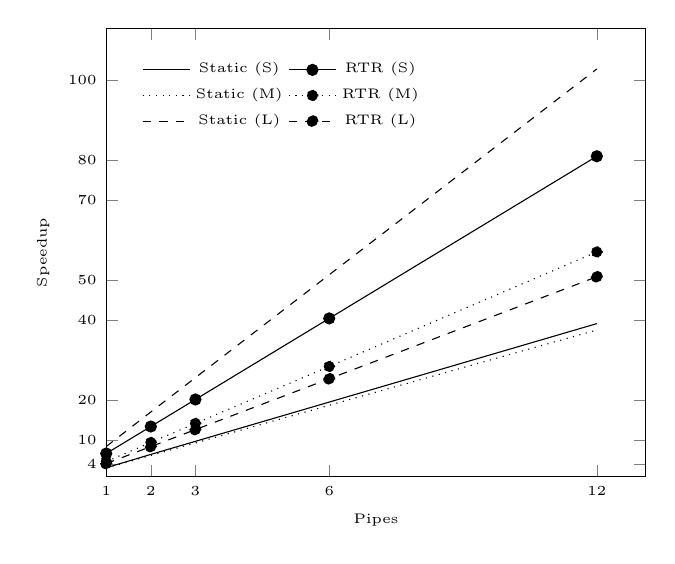
\begin{tikzpicture}
    \selectcolormodel{gray}
    \begin{axis}[
        xmin=1,
        ymin=1,
        %no markers,
        font=\tiny,
        xlabel=Pipes,
        ylabel=Speedup,
        xtick={1,2,3,6,12},
        ytick={4, 10, 20, 40, 50, 70, 80, 100},
        legend columns=2,
        legend entries={
          Static (S),
          RTR (S),
          Static (M),
          RTR (M),
          Static (L),
          RTR (L)},
        legend style={
          draw=none,
          at={(0.05,0.85) },
          anchor=west
        }
      ]

      \addplot[mark=none] coordinates {
        (1, 3.2)
        (2, 6.53)
        (3, 9.8)
        (6, 19.6)
        (12, 39.2)
      };
      \addplot[mark=*] coordinates {
        (1, 6.75)
        (2, 13.5)
        (3, 20.25)
        (6, 40.5)
        (12, 81)
      };
      \addplot[dotted] coordinates {
        (1, 3.13)
        (2, 6.26)
        (3, 9.4)
        (6, 18.8)
        (12, 37.6)
      };
      \addplot[mark=*, dotted] coordinates {
        (1, 4.75)
        (2, 9.51)
        (3, 14.27)
        (6, 28.5)
        (12, 57.1)
      };
      \addplot[mark=none, dashed] coordinates {
        (1, 8.5)
        (2, 17.13)
        (3, 25.7)
        (6, 51.4)
        (12, 102.8)
      };
      \addplot[mark=*, dashed] coordinates {
        (1, 4.25)
        (2, 8.48)
        (3, 12.725)
        (6, 25.42)
        (12, 50.9)
      };2
    \end{axis}
  \end{tikzpicture}
  \caption{Scalability of the RTM dataflow design explored using the aspect
shown in Fig.~\ref{fig:aspect-exploration}.}
  \label{fig:scalability}
  \vspace{-2mm}
\end{figure}

Fig.~\ref{fig:scalability} also shows the performance benefits of
using a run-time reconfiguration implementation which is generated by
using the reconfiguration aspect of Fig. 4 to create two
configurations for the RTM MaxC kernel. Since during the first half of
the execution the backward propagation and imaging functions are idle,
the first configuration requires only half the resources. This allows
doubling the number of parallel pipelines and halves the execution
time of the first configuration. The speedup obtained is comparable to
\cite{Xinyu:Qiwei:Luk:Qiang:Pell:2012}, but the partitioning and
optimisation exploration process is automated via aspects, which
increases developer productivity. The automated process improves
portability of the design, allowing optimisations based on design
space exploration to be carried out on various platforms (hence
subject to varying resource constraints) without manual intervention.

\section{Related Work}

A number of dataflow languages have been developed targeting FPGAs but
also multi-core platforms. Table \ref{table:feature-comparison}
summarizes some of the important features of these languages compared
to MaxC. Lucid \cite{ashcroft1977lucid}, SISAL
\cite{gurd1987implicit}, \cite{mcgraw1983sisal} and Lustre
\cite{halbwachs1991synchronous}, are examples of functional dataflow
languages. The latter is based on a synchronous programming model,
facilitating safety verification for critical software
\cite{halbwachs1992programming} rather than performance. The
functional programming style complicates the translation of existing
imperative applications and none have existing implementations for
FPGAs, so a performance comparison is not possible.
Streams-C\cite{Gokhale:Stone:Arnold:Kalinowski:2000} and
ImpulseC\cite{ImpulseC} use imperative ANSI C syntax and an execution
model based on Communicating Sequential Processes and introduce
non-standard syntax and constructs for specifying designs such as
special comment blocks which are used to annotate the C application
code. This makes the languages harder to integrate with existing
source-to-source translation or aspect weaving frameworks. Hybrid
approaches such as MaxCompiler \cite{MaxelerTechnologies:2012}
separate the CPU runtime component from the accelerated one, providing
an imperative C based runtime environment and a Java dataflow API for
building the accelerator designs. This separation complicates the
development process, since the two components have to be managed
separately and hinders information sharing between the two components
(such as common design parameters) and, consequently, the design space
exploration process.

\begin{table}[!h]
  \renewcommand{\arraystretch}{1.2}
  \centering
  \caption{Feature comparison of MaxC and other dataflow languages.}
  \label{table:feature-comparison}
  \begin{tabular}{ c |  c |  c |  c |  c }
    \hline
    \         & \bf{Syntax} & \bf{Paradigm} & \bf{Impl.} & \bf{Support} \\
    \hline \hline
    Lucid     & Lucid       & Func.         & Multiproc. & Software     \\
    SISAL     & SISAL       & Func.         & Multiproc. & Software     \\
    Lustre    & Lustre      & Sync.         & Multiproc. & Software     \\
    MaxJ      & Java        & Imp.          & FPGA       & Hardware     \\
    Streams-C & C           & Imp./CSP      & FPGA       & Combined     \\
    ImpulseC  & C           & Imp./CSP      & Both       & Combined     \\
    MaxC      & C           & Imp.          & FPGA       & Combined     \\
  \end{tabular}
\end{table}

The use of LARA aspects in guiding the compilation process of C
application is also described in
\cite{Cardoso:Teixeira:Alves:Nobre:Diniz:Cutinho:Luk:2012} and
\cite{cardoso2011new} but the backend compilation targets a von
Neumann architecture (GPP + custom accelerator units) unlike the
dataflow architecture proposed in this paper. The approach described
in \cite{Cardoso:Teixeira:Alves:Nobre:Diniz:Cutinho:Luk:2012} and
\cite{cardoso2011new} relies more on high-level source transformation
whereas our approach is based on a more systematic design level
exploration process, which enables the analysis of more low-level
optimisations. Finally,
\cite{Cardoso:Teixeira:Alves:Nobre:Diniz:Cutinho:Luk:2012} and
\cite{cardoso2011new} do not consider development aspects which can be
used to improve developer productivity and run-time reconfiguration
aspects that can lead to improved performance.

The use of aspect-oriented programming for specifying strategies for
run-time adaptation of FPGA designs is discussed in
\cite{6322875}. This is different than the static process considered
in this paper in which the run-time reconfiguration aspects generate
and schedule all partitions of the application at compile time, to
achieve optimal performance as described in
\cite{Xinyu:Qiwei:Luk:Qiang:Pell:2012}. One advantage of our approach
is that an optimal allocation is generated from the start. However we
do not have the flexibility of adapting the design to varying input
conditions.

\section{Conclusion}

In this paper we present an automated design flow for design space
exploration of dataflow designs based on a novel language, MaxC, and
aspect-driven compilation. We show that this approach meets the
initial performance, portability, integration and productivity
requirements. We implement a high performance dataflow design for RTM
to show that we can achieve significant speedups over software only
versions by exploiting the run-time reconfiguration. The automated
aspect-driven optimisation process improves productivity and design
portability, allowing optimisations strategies to be automatically
adapted to various platforms.  Finally we show that MaxC is a concise
language and that maintaining compatibility with C99 simplifies the
translation of existing applications.

Future work includes extending our approach by introducing new system
aspects that guide the translation and optimisation process from
existing C applications to dataflow designs. This includes the
development of system aspects that can be used to explore structural
transformations of the original application that improve parallelism
and computation versus communication ratio. The introduction of these
aspects could lead to a transparent design flow, that does not require
manual development of dataflow designs, greatly simplifying the
translation of existing software applications to high-performance
custom designs.


% Note that IEEE typically puts floats only at the top, even when this
% results in a large percentage of a column being occupied by floats.


% An example of a double column floating figure using two subfigures.
% (The subfig.sty package must be loaded for this to work.)
% The subfigure \label commands are set within each subfloat command, the
% \label for the overall figure must come after \caption.
% \hfil must be used as a separator to get equal spacing.
% The subfigure.sty package works much the same way, except \subfigure is
% used instead of \subfloat.
%

% Note that often IEEE papers with subfigures do not employ subfigure
% captions (using the optional argument to \subfloat), but instead will
% reference/describe all of them (a), (b), etc., within the main caption.


% An example of a floating table. Note that, for IEEE style tables, the
% \caption command should come BEFORE the table. Table text will default to
% \footnotesize as IEEE normally uses this smaller font for tables.
% The \label must come after \caption as always.
%
%\begin{table}[!t]
%% increase table row spacing, adjust to taste
%\renewcommand{\arraystretch}{1.3}
% if using array.sty, it might be a good idea to tweak the value of
% \extrarowheight as needed to properly center the text within the cells
%\caption{An Example of a Table}
%\label{table_example}
%\centering
%% Some packages, such as MDW tools, offer better commands for making tables
%% than the plain LaTeX2e tabular which is used here.
%\begin{tabular}{|c||c|}
%\hline
%One & Two\\
%\hline
%Three & Four\\
%\hline
%\end{tabular}
%\end{table}


% Note that IEEE does not put floats in the very first column - or typically
% anywhere on the first page for that matter. Also, in-text middle ("here")
% positioning is not used. Most IEEE journals/conferences use top floats
% exclusively. Note that, LaTeX2e, unlike IEEE journals/conferences, places
% footnotes above bottom floats. This can be corrected via the \fnbelowfloat
% command of the stfloats package.


\section*{Acknowledgment}

This work is supported in part by the China Scholarship Council, by
the European Union Seventh Framework Programme under grant agreement
number 257906, 287804 and 318521, by UK EPSRC, by Maxeler University
Programme, and by Xilinx.

% trigger a \newpage just before the given reference
% number - used to balance the columns on the last page
% adjust value as needed - may need to be readjusted if
% the document is modified later
%\IEEEtriggeratref{0}
% The "triggered" command can be changed if desired:
%\IEEEtriggercmd{\enlargethispage{-5in}}

\bibliographystyle{IEEEtran}
\bibliography{../../refdb/bibliography.bib}



\end{document}
